% The width shortfall: the flat fit is fitted to the centre rows only, so the
% width rows are a held-out comparison. Medians agree by construction; the gap
% in spread is the diagnostic.
%
%   compile:  pdflatex width_shortfall.tex
%
\documentclass[border=10pt]{standalone}
\usepackage{lmodern}
\usepackage{amsmath}
\usepackage{amssymb}
\usepackage{tikz}
\usetikzlibrary{arrows.meta,positioning,decorations.pathreplacing}
% Shared palette for the population-model figures.
%   ink      body / structure
%   popcol   the patient cloud and anything predicted from it
%   mechcol  the simulator and species-level quantities
%   msrcol   the measurement map (readout-level: gamma, kappa)
%   datacol  reported rows
\definecolor{ink}{HTML}{3A3A3A}
\definecolor{popcol}{HTML}{3B4AA6}
\definecolor{mechcol}{HTML}{2E7D5B}
\definecolor{msrcol}{HTML}{EB811B}
\definecolor{datacol}{HTML}{8C3B4A}


\begin{document}
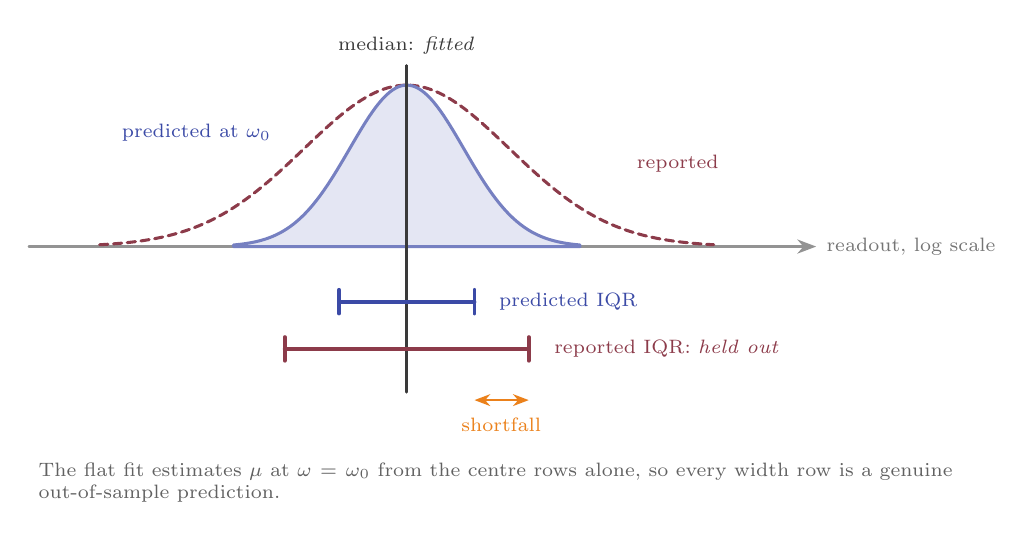
\begin{tikzpicture}[
  font=\sffamily, >=Stealth, line cap=round, line join=round,
  figcap/.style={font=\scriptsize, text=ink!80, align=left, anchor=north west}]

\def\m{5.2}

% ---- axis -------------------------------------------------------------
\draw[ink!55, line width=0.8pt, -{Stealth[length=2.4mm]}] (0.4,0) -- (10.4,0)
  node[right, font=\scriptsize, ink!70] {readout, log scale};

% ---- reported spread (what the cohort's quartiles imply) --------------
\draw[datacol, line width=1.1pt, densely dashed]
  plot[domain=1.3:9.1,samples=110,smooth] (\x,{2.05*exp(-(\x-\m)*(\x-\m)/3.4)});
\node[datacol, font=\scriptsize, anchor=west] at (8.0,1.05) {reported};

% ---- predicted cloud at omega_0 ---------------------------------------
\draw[popcol!70, fill=popcol!14, line width=1.1pt]
  plot[domain=3.0:7.4,samples=110,smooth] (\x,{2.05*exp(-(\x-\m)*(\x-\m)/1.05)})
  -- (7.4,0) -- (3.0,0) -- cycle;
\node[popcol, font=\scriptsize, anchor=east] at (3.6,1.45) {predicted at $\omega_0$};

% ---- the matched centre ------------------------------------------------
\draw[ink, line width=1pt] (\m,-1.85) -- (\m,2.30);
\node[ink, font=\scriptsize, anchor=south] at (\m,2.32)
  {median: \emph{fitted}};

% ---- the two widths ----------------------------------------------------
\draw[popcol, line width=1.4pt] (\m-0.86,-0.70) -- (\m+0.86,-0.70);
\draw[popcol, line width=1.4pt] (\m-0.86,-0.85) -- (\m-0.86,-0.55);
\draw[popcol, line width=1.4pt] (\m+0.86,-0.85) -- (\m+0.86,-0.55);
\node[popcol, font=\scriptsize, anchor=west] at (\m+1.05,-0.70) {predicted IQR};

\draw[datacol, line width=1.4pt] (\m-1.55,-1.30) -- (\m+1.55,-1.30);
\draw[datacol, line width=1.4pt] (\m-1.55,-1.45) -- (\m-1.55,-1.15);
\draw[datacol, line width=1.4pt] (\m+1.55,-1.45) -- (\m+1.55,-1.15);
\node[datacol, font=\scriptsize, anchor=west] at (\m+1.75,-1.30) {reported IQR: \emph{held out}};

% ---- the shortfall ------------------------------------------------------
\draw[msrcol, line width=1pt, {Stealth[length=2mm]}-{Stealth[length=2mm]}]
  (\m+0.86,-1.95) -- (\m+1.55,-1.95);
\node[msrcol, font=\scriptsize, anchor=north] at (\m+1.20,-2.05) {shortfall};

\node[figcap, text width=118mm] at (0.4,-2.62)
  {The flat fit estimates $\mu$ at $\omega=\omega_0$ from the centre rows alone, so every
   width row is a genuine out-of-sample prediction.};

\end{tikzpicture}
\end{document}
